\subsection{The committed documents reproduced, and the first four statements}
\label{sec:results-reproduction}

The Annex 1 treatment of the code of this paper, run on the flows and the curves of the case at the committed seed, reproduces the committed delta EVE, delta NII, indexation charge and twelve-month margin of each of the six variants with a largest relative deviation of \repMaxDev{}, and the leg deltas of every scenario agree with the committed pairs; Table~\ref{tab:reproduction} lists the committed measures. The reproduction is a contract test of the module and also fixes the reading of the case: the delta NII of the long UF variant is \repAnnexNiiLng{} million pesos, of which the charge is \repChargeLng{} and the largest pair \repMaxPairLng{}, and its delta EVE is \repAnnexEveLng{}, \repEveTLng{} percent of level 1 capital.

\begin{table}[htbp]
\centering
\footnotesize
\setlength{\tabcolsep}{3.5pt}
\caption{The six variants of case C15 as committed (seed 42, valuation date 2026-09-03, CLP million): the delta NII and delta EVE of the Annex 1 treatment, the indexation charge as a share of the delta NII, the smallest distance between a post-shock rate and its floor, and the largest relative deviation between the committed measures and the measures recomputed here from the same flows by independent engine calls.}
\label{tab:reproduction}
\begin{tabular}{lrrrrrr}
\toprule
Variant & Net UF / $T_1$ & $\Delta$NII & $\Delta$EVE & Charge / $\Delta$NII & Closest floor (bp) & Max relative deviation \\
\midrule
Long UF & 30\% & 11{,}213 & 93{,}816 & 55.1\% & 20.48 & 0e+00 \\
Short UF & $-$30\% & 11{,}067 & 79{,}643 & 55.9\% & 20.48 & 0e+00 \\
CPI surprise & 30\% & 11{,}213 & 93{,}816 & 55.1\% & 20.48 & 0e+00 \\
CLP steepener & 5\% & 6{,}783 & 140{,}645 & 15.2\% & 20.48 & 0e+00 \\
Offset on and off & 30\% & 11{,}016 & 81{,}173 & 56.1\% & 20.48 & 0e+00 \\
Floor-exposed & 5\% & 6{,}606 & 60{,}764 & 15.6\% & 20.48 & 0e+00 \\
\bottomrule
\end{tabular}
\end{table}


The four statements of the design document are reproduced. R1: the indexation charge is \repChargeShareSht{} percent of the delta NII of the short UF variant, and \repChargeShareLo{} to \repChargeShareHi{} percent in the three variants with a 30 percent position. R2: the single-currency treatment of the same flows gives a delta NII of \repSingleNiiLng{}, \repSingleNiiSht{} and \repSingleNiiOff{} million pesos in the long UF, short UF and offset variants against \repAnnexNiiLng{}, \repAnnexNiiSht{} and \repAnnexNiiOff{}, that is \repRatioLo{} to \repRatioHi{} times smaller. R3: its delta EVE is \repSingleEveLng{}, \repSingleEveSht{} and \repSingleEveOff{} against \repAnnexEveLng{}, \repAnnexEveSht{} and \repAnnexEveOff{}, \repEveShortLo{} to \repEveShortHi{} percent smaller. R4: the smallest distance between a post-shock rate and its floor is \repFloorDistLng{} basis points in every variant, so no floor binds. Figure~\ref{fig:curves} shows why: the UF curve after a fall of 300 basis points, the largest shock of the income measure, stays above the floor of minus two percent at the short end by that margin. The classification under the three prioritisation tests is the same under every treatment in the six variants, and only the CLP steepener variant is flagged, by the value test, with a delta EVE of \repEveTStp{} percent of level 1 capital under Annex 1 and \repEveTSingleStp{} percent under the single-currency treatment.

\begin{figure}[htbp]
\centering
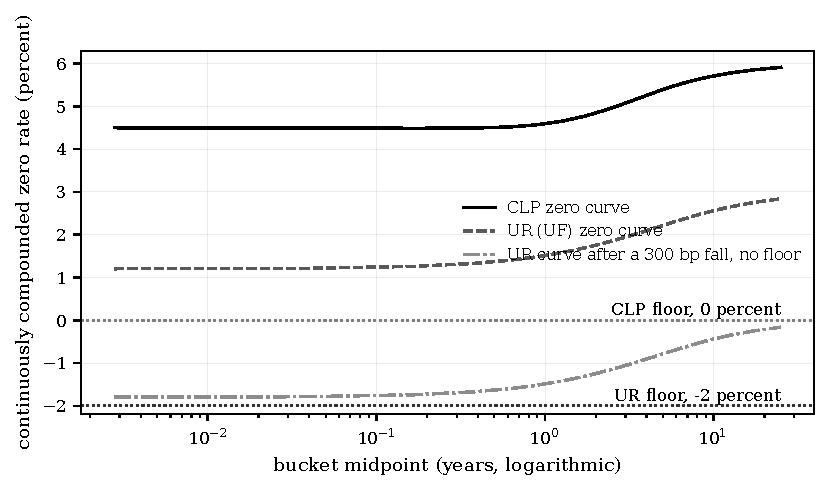
\includegraphics[width=0.78\textwidth]{curves-and-floors}
\caption{The two zero curves fitted by the engine to the Banco Central de Chile yields of 2026-09-03 at the 19 bucket midpoints, the UF curve after a parallel fall of 300 basis points without a floor, and the floors of the two currencies, minus 2 percent for the UF and 0 for the peso; the lowest point of the fallen UF curve is the smallest distance to a floor in the committed documents.}
\label{fig:curves}
\end{figure}

\subsection{The main comparison}
\label{sec:results-main}

Table~\ref{tab:main-results} compares the treatments on 30 books of each of the three variants whose net UF position is 30 percent of level 1 capital. The Annex 1 delta NII is $\mainAnnexNiiLng\pm\mainAnnexNiiLngCi$, $\mainAnnexNiiSht\pm\mainAnnexNiiShtCi$ and $\mainAnnexNiiOff\pm\mainAnnexNiiOffCi$ million pesos, about \mainAnnexNiiTLng{} percent of level 1 capital. The single-currency delta NII is $\mainSingleNiiLng\pm\mainSingleNiiLngCi$, $\mainSingleNiiSht\pm\mainSingleNiiShtCi$ and $\mainSingleNiiOff\pm\mainSingleNiiOffCi$, so the Annex 1 measure is $\mainRatioNiiLng\pm\mainRatioNiiLngCi$, $\mainRatioNiiSht\pm\mainRatioNiiShtCi$ and $\mainRatioNiiOff\pm\mainRatioNiiOffCi$ times larger. These ratios are below those of the committed seed, \repRatioLo{} to \repRatioHi{}: the committed book lies in the upper part of the distribution over books, and the range quoted by the design document is the range of that one book, not of the treatment. The Basel positive-part aggregation gives about three quarters of the Annex 1 income measure (\mainPosOverAnnexNiiLng{}, \mainPosOverAnnexNiiSht{} and \mainPosOverAnnexNiiOff{}), because it has no charge; the earnings gap of the whole book equals the single-currency income measure to the unit in every row, the identity of Section~\ref{sec:method-implementation}. The charge supplies $\mainChargeShareLng\pm\mainChargeShareLngCi$, $\mainChargeShareSht\pm\mainChargeShareShtCi$ and $\mainChargeShareOff\pm\mainChargeShareOffCi$ percent of the Annex 1 income measure.

\begin{table}[htbp]
\centering
\footnotesize
\setlength{\tabcolsep}{3.5pt}
\caption{Main comparison on the three variants whose net UF position is 30 percent of level 1 capital: the delta NII and the delta EVE of the Annex 1 treatment, of the positive-part aggregation of the Basel standard, of the single-currency treatment of the same flows, and of the repricing-gap and duration-gap measures, as the mean and the half-width of the 95 percent Student interval over 30 synthetic books (seeds 1 to 30) on the curves of 2026-09-03; the three right columns divide each mean by the Annex 1 mean.}
\label{tab:main-results}
\begin{tabular}{lrrrrrr}
\toprule
\multicolumn{7}{l}{\textbf{Panel A. Delta NII, CLP million (left: mean $\pm$ 95\% half-width; right: ratio to Annex 1)}} \\
\midrule
Treatment & Long UF & Short UF & Offset on/off & Long UF & Short UF & Offset \\
\midrule
Annex 1 (separate UR) & 11{,}907$\pm$251 & 11{,}772$\pm$252 & 11{,}725$\pm$252 & 1.00 & 1.00 & 1.00 \\
Positive parts (Basel aggregation) & 9{,}039$\pm$230 & 9{,}039$\pm$230 & 9{,}039$\pm$230 & 0.76 & 0.77 & 0.77 \\
Single currency & 2{,}412$\pm$323 & 2{,}143$\pm$325 & 2{,}049$\pm$325 & 0.20 & 0.18 & 0.17 \\
Repricing gap (single currency) & 2{,}412$\pm$323 & 2{,}143$\pm$325 & 2{,}049$\pm$325 & 0.20 & 0.18 & 0.17 \\
\midrule
\multicolumn{7}{l}{\textbf{Panel B. Delta EVE, CLP million (left: mean $\pm$ 95\% half-width; right: ratio to Annex 1)}} \\
\midrule
Treatment & Long UF & Short UF & Offset on/off & Long UF & Short UF & Offset \\
\midrule
Annex 1 (separate UR) & 85{,}061$\pm$1{,}875 & 68{,}605$\pm$2{,}088 & 72{,}044$\pm$1{,}824 & 1.00 & 1.00 & 1.00 \\
Positive parts (Basel aggregation) & 85{,}927$\pm$1{,}810 & 68{,}605$\pm$2{,}088 & 85{,}434$\pm$1{,}792 & 1.01 & 1.00 & 1.19 \\
Single currency & 80{,}186$\pm$1{,}790 & 58{,}057$\pm$1{,}827 & 54{,}645$\pm$1{,}758 & 0.94 & 0.85 & 0.76 \\
Duration gap (single currency) & 91{,}126$\pm$2{,}178 & 64{,}216$\pm$2{,}251 & 59{,}621$\pm$2{,}155 & 1.07 & 0.94 & 0.83 \\
\bottomrule
\end{tabular}
\end{table}


For the value measure the single-currency treatment is $\mainEveShortLng\pm\mainEveShortLngCi$, $\mainEveShortSht\pm\mainEveShortShtCi$ and $\mainEveShortOff\pm\mainEveShortOffCi$ percent below Annex 1. The long UF variant has the smallest shortfall and the offset variant the largest; in the offset variant the two legs move in opposite directions at several scenarios, so that the Basel positive-part aggregation is \mainPosOverAnnexEveOff{} times the Annex 1 measure, the only case in which it differs from it by more than one percent (\mainPosOverAnnexEveLng{} and \mainPosOverAnnexEveSht{} in the other two). The duration gap, a first-order measure of the whole book as one currency, gives \mainGapOverAnnexEveLng{}, \mainGapOverAnnexEveSht{} and \mainGapOverAnnexEveOff{} times the Annex 1 value measure: it is above it for the long UF book and below it for the other two, so a first-order single-currency measure does not have a stable sign against the supervisor's measure. Figure~\ref{fig:main} gives the six variants as a share of level 1 capital. The steepener and floor-exposed variants have a net UF position of 5 percent of level 1 capital and so a small charge; their income ratios, \mainRatioNiiStp{} and \mainRatioNiiFlr{}, are smaller than those of the 30 percent variants, in line with Proposition~\ref{prop:charge}.

\begin{figure}[htbp]
\centering
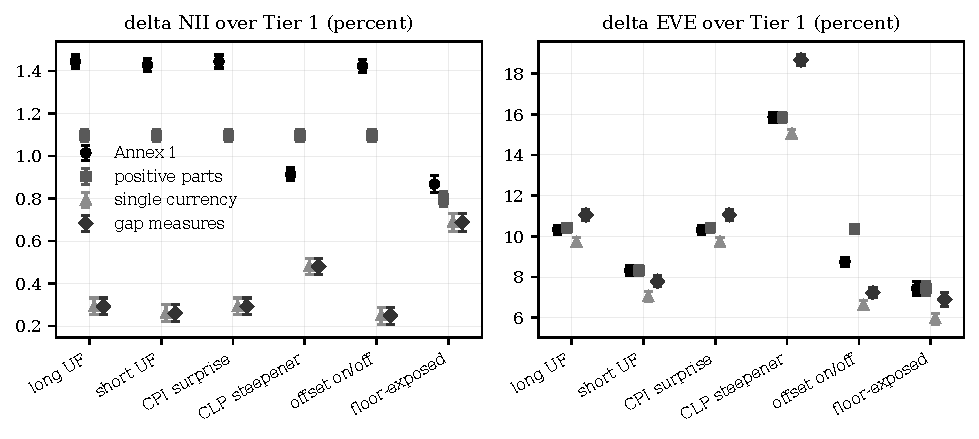
\includegraphics[width=\textwidth]{treatments-over-tier1}
\caption{Delta NII (left) and delta EVE (right) as a percentage of level 1 capital under the Annex 1 treatment, the Basel positive-part aggregation, the single-currency treatment and the repricing-gap and duration-gap measures, for the six variants; points are means over 30 synthetic books and bars are 95 percent half-widths.}
\label{fig:main}
\end{figure}

\subsection{The bound and the first predictions}
\label{sec:results-hypotheses}

H1 holds. In \hOneChecked{} comparisons over six variants, 30 books, eight combinations of curve, sizes and floor, and the two measures, and in \repSandChecked{} further comparisons on the committed seed, there are \hOneViol{} violations of the order $N\le P_{1/2}\le Q$ of Proposition~\ref{prop:pair} (\repSandViol{} on the committed seed). Figure~\ref{fig:pair} draws the three aggregation rules for two legs, one gaining and one losing, from the engine's \texttt{cmf\_pair}: the pair rule lies between the other two and reduces the positive-part sum by at most half of the gain.

\begin{figure}[htbp]
\centering
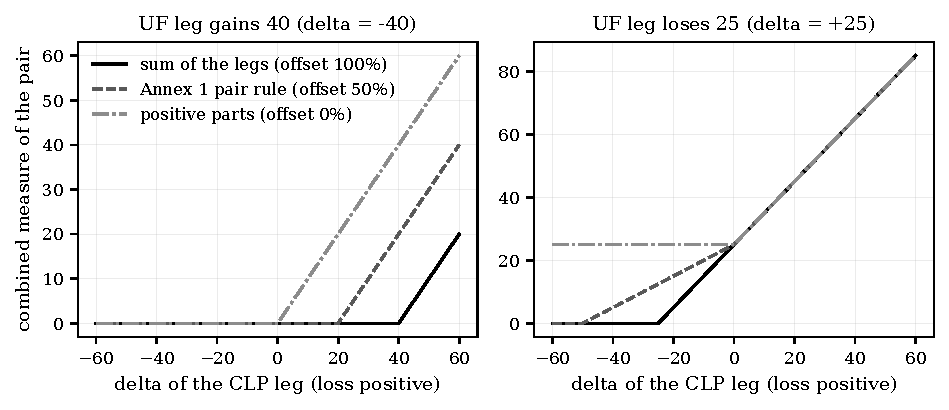
\includegraphics[width=0.92\textwidth]{pair-function}
\caption{The aggregation of the two legs' deltas as a function of the delta of the peso leg, for a UF leg that gains 40 (left) and one that loses 25 (right): the sum of the legs, the pair rule of Annex 1 with a 50 percent offset computed by the engine's cmf\_pair, and the sum of the positive parts used by the Basel standard.}
\label{fig:pair}
\end{figure}

H2 is refuted. In the three variants with a 30 percent position the switch with the largest absolute Shapley value for the delta EVE is the \hTwoTopLng{} in each, not the pair rule (Section~\ref{sec:ablation}). H3 is refuted in one clause: in the CLP steepener variant the Annex 1 delta NII is below the Basel positive-part one in \hThreeSteeperViol{} of 30 books, \mainPosOverAnnexNiiStp{} times larger for the positive parts. Equation~\eqref{eq:charge-condition} gives the reason: the positive part \repPosNiiStp{} exceeds the largest pair \repMaxPairStp{} by more than the charge \repChargeStp{}, because the net UF position is only \repNuStp{} percent of level 1 capital; in the other five variants this clause holds in every book, and the other two clauses of H3 hold in all 180 books. The own curve is also the reason for a result of the theory that the data show directly: discounting the UF assets on the peso curve understates their present value by \repAssetUnderLng{} percent in the committed book, and the UF liabilities of the short UF book by \repLiabUnderSht{} percent, since the discount factor on the peso curve is \dfRatioFive{}, \dfRatioTen{} and \dfRatioLast{} times that on the UF curve at 5.5, 9.5 and 25 years (Figure~\ref{fig:fisher}).

\begin{figure}[htbp]
\centering
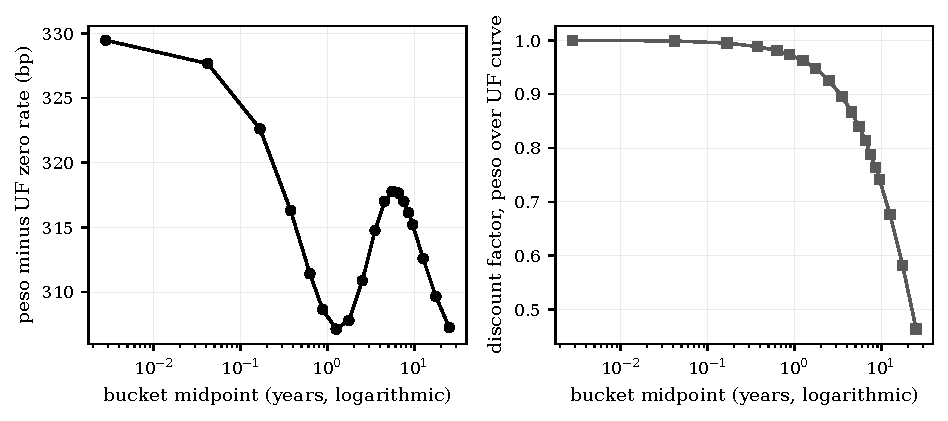
\includegraphics[width=0.92\textwidth]{peso-curve-on-uf-flows}
\caption{The gap between the peso and the UF zero rate (left) and the ratio of the discount factor on the peso curve to the one on the UF curve (right) at the 19 bucket midpoints, from the curves of 2026-09-03; the ratio is the factor by which a peso curve understates the value of an indexed flow.}
\label{fig:fisher}
\end{figure}

\subsection{When the two treatments classify a bank differently}
\label{sec:results-sweep}

Figure~\ref{fig:sweep} and Table~\ref{tab:sweep} give the two measures as a share of level 1 capital against the net UF position of the long UF book, from \sweepLo{} to \sweepHi{} percent; the generator refuses the other \sweepRefused{} of the 31 positions of the grid, those that would need more UF borrowings than the book has. At the position of the committed variants, 30 percent, the Annex 1 income measure is \swThreeAnnexNii{} percent of level 1 capital and the single-currency one \swThreeSingleNii{} percent; the value measures are \swThreeAnnexEve{} and \swThreeSingleEve{} percent. No book is flagged by any treatment up to a position of 50 percent. The Basel positive-part aggregation flags its first books at \sweepPosFlagFirst{} percent, the Annex 1 treatment flags \swTenFlagAnnex{} of 20 books at 100 percent, \swElevenFlagAnnex{} at 110 percent and \swFifteenFlagAnnex{} at 150, while the single-currency treatment flags none up to 110 percent, \swTwelveFlagSingle{} at 120 percent and \swFifteenFlagSingle{} at 150 percent (Figure~\ref{fig:flags}).

\begin{figure}[htbp]
\centering
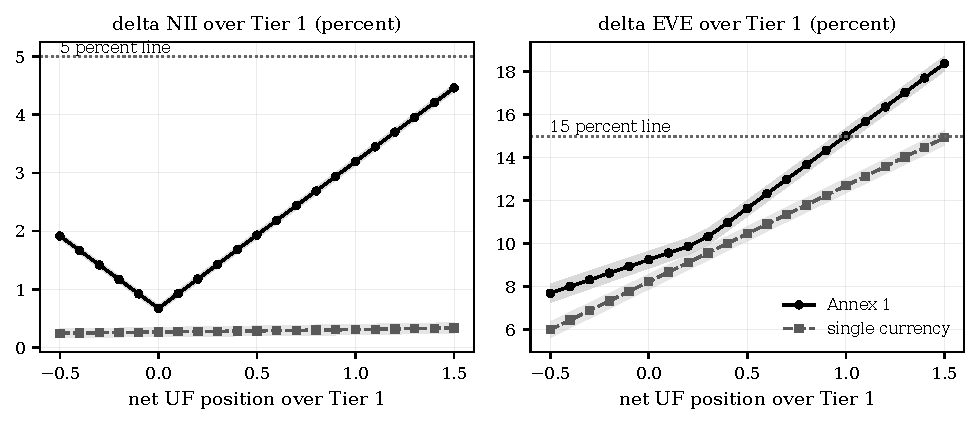
\includegraphics[width=\textwidth]{position-sweep}
\caption{Delta NII (left) and delta EVE (right) as a percentage of level 1 capital against the net UF position, for the Annex 1 and the single-currency treatments, with the 5 and 15 percent prioritisation lines; lines are means over 20 synthetic books and bands are 95 percent intervals.}
\label{fig:sweep}
\end{figure}

\begin{table}[htbp]
\centering
\footnotesize
\setlength{\tabcolsep}{3.5pt}
\caption{The delta NII (NII) and delta EVE (EVE) as a share of level 1 capital under the Annex 1 (A1) and the single-currency (SC) treatments, and the number of the 20 synthetic books (seeds 101 to 120) that Annex 1 (Flag A1), the positive-part aggregation (Flag PP) and the single currency (Flag SC) flag as prioritised under at least one of the three tests of Annex 1, at selected net UF positions of the long UF book (positive: UF assets exceed UF funding).}
\label{tab:sweep}
\begin{tabular}{lrrrrrrr}
\toprule
Net UF / $T_1$ & NII A1 & NII SC & EVE A1 & EVE SC & Flag A1 & Flag PP & Flag SC \\
\midrule
$-$50\% & 1.92\% & 0.25\% & 7.7\% & 6.0\% & 0 & 0 & 0 \\
0\% & 0.67\% & 0.27\% & 9.2\% & 8.2\% & 0 & 0 & 0 \\
30\% & 1.43\% & 0.28\% & 10.3\% & 9.6\% & 0 & 0 & 0 \\
80\% & 2.69\% & 0.30\% & 13.7\% & 11.8\% & 1 & 17 & 0 \\
100\% & 3.19\% & 0.31\% & 15.0\% & 12.7\% & 10 & 20 & 0 \\
110\% & 3.45\% & 0.32\% & 15.7\% & 13.1\% & 17 & 20 & 0 \\
120\% & 3.70\% & 0.32\% & 16.4\% & 13.6\% & 19 & 20 & 1 \\
150\% & 4.46\% & 0.34\% & 18.4\% & 14.9\% & 20 & 20 & 8 \\
\bottomrule
\end{tabular}
\end{table}


H4 holds, narrowly: there are \hFourN{} positions, from \hFourLo{} to \hFourHi{} percent of level 1 capital, at which Annex 1 flags more than half of the books and the single-currency treatment flags none or few. Three qualifications bound the result. The flag is the value test, of 15 percent of level 1 capital, in every case: the income test is never breached by any treatment at any position (the largest mean income measure is \sweepMaxAnnexNii{} percent, below the 5 percent line, and the number of flags of the income tests is \sweepNiiFlagTotal{} and of the margin test \sweepMarginFlagTotal{}), consistent with Proposition~\ref{prop:charge}, which needs a position of \floorBreakNu{} times level 1 capital for the charge alone to breach. The positions are large, a net UF position above the whole of the capital. And the Basel positive-part aggregation flags earlier than either, so that the differing classification is mainly the effect of the pair rule and of the sizes on the value measure and not of the indexation charge.

\begin{figure}[htbp]
\centering
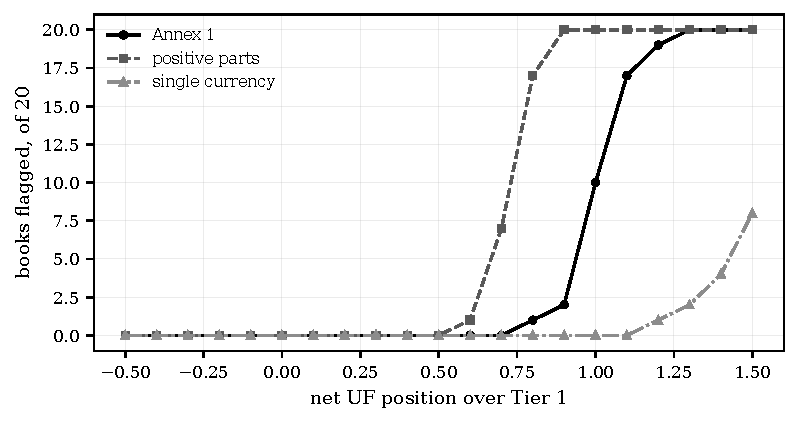
\includegraphics[width=0.78\textwidth]{prioritised-flags}
\caption{The number of the 20 synthetic books flagged as prioritised under at least one of the three tests of Annex 1 against the net UF position, for the Annex 1 treatment, the Basel positive-part aggregation and the single-currency treatment.}
\label{fig:flags}
\end{figure}

\subsection{The floor of the UF made to bind}
\label{sec:results-floors}

On the curves of the valuation date the distance of the lowest post-shock UF rate to its floor is \floorsDistZero{} basis points, so the floor binds nowhere and its effect is not shown by the committed documents. Translating the UF curve down by 25 basis points puts the lowest rate \flTwentyFiveDistLng{} basis points past the floor; the effect on a measure then depends on the book (Table~\ref{tab:floors}, Figure~\ref{fig:floors}). On the delta EVE the floor changes the measure in \floorsEveChanged{} of the comparisons at every translation up to $-300$ basis points, because the scenario that attains the maximum is the parallel-up shock, on which a floor cannot bind. On the delta NII the effect of the floor in the long UF variant is zero up to a translation of 50 basis points, $\flHundredEffLng\pm\flHundredEffLngCi$ at $-100$, $\flTwoHundredEffLng\pm\flTwoHundredEffLngCi$ at $-200$ and $\flThreeHundredEffLng\pm\flThreeHundredEffLngCi$ million pesos at $-300$ basis points, and it is positive: the floor raises the measure, in \flThreeHundredRaiseLng{} of 20 books at $-300$ and in none lowers it. In the floor-exposed variant, whose UF leg is asset-sensitive because 70 percent of its commercial loans float, the floor lowers the measure at small translations (\flFiftyLowerFlr{} of 20 books at $-50$ basis points, mean effect $\flFiftyEffFlr\pm\flFiftyEffFlrCi$) and raises it at large ones (\flThreeHundredRaiseFlr{} of 20 at $-300$, mean $\flThreeHundredEffFlr\pm\flThreeHundredEffFlrCi$).

\begin{table}[htbp]
\centering
\footnotesize
\setlength{\tabcolsep}{3.5pt}
\caption{The UR floor of minus 2 percent made to bind by translating the fitted UF zero curve down: the mean distance of the lowest post-shock UR rate to the floor (negative once it binds), the Annex 1 delta NII without any floor and with the floor, the effect of the floor with its 95 percent half-width, and the number of the 20 books (seeds 201 to 220) in which the floor raises or lowers the measure, for two variants.}
\label{tab:floors}
\begin{tabular}{lrrrrrr}
\toprule
\multicolumn{7}{l}{\textbf{Panel A. Delta NII, long uf variant, CLP million}} \\
\midrule
Shift (bp) & Dist. (bp) & No floor & Floor & Effect & Raised & Lowered \\
\midrule
+0 & 20.5 & 11{,}711 & 11{,}711 & 0$\pm$0 & 0 & 0 \\
$-$25 & -4.5 & 11{,}711 & 11{,}711 & 0$\pm$0 & 0 & 0 \\
$-$50 & -29.5 & 11{,}711 & 11{,}711 & 0$\pm$0 & 0 & 0 \\
$-$100 & -79.5 & 11{,}711 & 11{,}719 & 8$\pm$16 & 1 & 0 \\
$-$200 & -179.5 & 11{,}711 & 11{,}832 & 120$\pm$156 & 6 & 0 \\
$-$300 & -279.5 & 11{,}711 & 12{,}392 & 681$\pm$404 & 11 & 0 \\
\midrule
\multicolumn{7}{l}{\textbf{Panel B. Delta NII, floor-exposed variant, CLP million}} \\
\midrule
Shift (bp) & Dist. (bp) & No floor & Floor & Effect & Raised & Lowered \\
\midrule
+0 & 20.5 & 7{,}041 & 7{,}041 & 0$\pm$0 & 0 & 0 \\
$-$25 & -4.5 & 7{,}041 & 7{,}041 & 0$\pm$0 & 0 & 0 \\
$-$50 & -29.5 & 7{,}041 & 7{,}022 & $-$19$\pm$15 & 2 & 18 \\
$-$100 & -79.5 & 7{,}041 & 7{,}100 & 58$\pm$40 & 15 & 5 \\
$-$200 & -179.5 & 7{,}041 & 7{,}256 & 215$\pm$90 & 16 & 4 \\
$-$300 & -279.5 & 7{,}041 & 7{,}413 & 372$\pm$140 & 17 & 3 \\
\bottomrule
\end{tabular}
\end{table}


\begin{figure}[htbp]
\centering
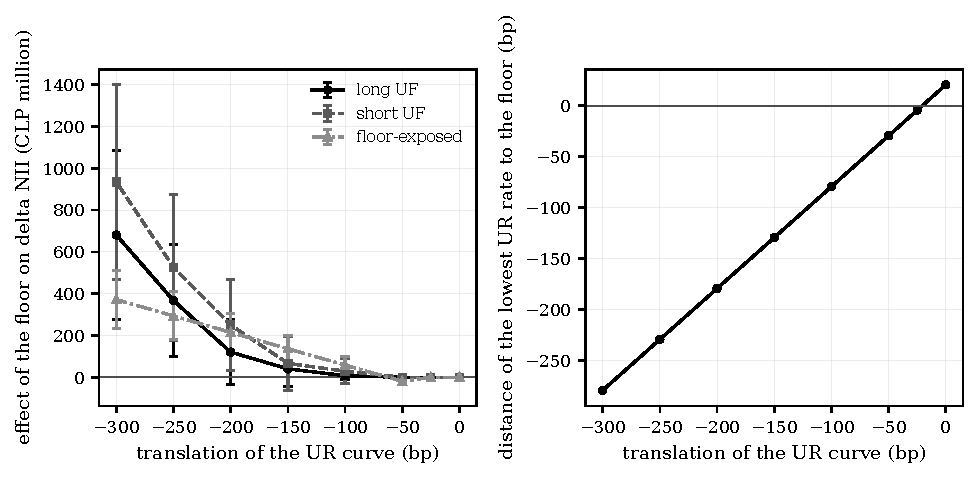
\includegraphics[width=\textwidth]{floor-effect}
\caption{Effect of the UF floor on the Annex 1 delta NII against the translation of the UF curve for three variants (left; means over 20 books with 95 percent intervals) and the distance of the lowest post-shock UF rate to the floor for the long UF variant (right).}
\label{fig:floors}
\end{figure}

H5 is refuted: \floorsRaise{} of \floorsTotal{} comparisons of the two measures over six variants, eight translations and 20 books show a measure with the floor above the measure without it, by up to \floorsMaxInc{} million pesos. The sign follows Proposition~\ref{prop:floor}: a liability-sensitive UF leg, as in the long UF, short UF and offset variants, has a gain in the falling scenario that the floor reduces, and the pair rule then offsets less of it against the peso loss. Across the five variants other than the floor-exposed one the floor lowers the measure in \floorsLowerOthers{} books, and in the floor-exposed one it lowers it in \floorsLowerTotalFlr{} and raises it in \floorsRaiseTotalFlr{} of the 160 book and translation pairs.
